%% cladograms.tex
%% Author: Leighton Pritchard
%% Copyright: James Hutton Institute
%% Introductory slides: Cladograms.

%
\begin{frame}
  \frametitle{Types of comparison}
    \begin{columns}[T] 
      \column{.5\textwidth} 
        \textcolor{RawSienna}{\textbf{Within species}}
        \begin{itemize}
	  \item e.g. isolate-level (and even within individuals)
	  \item which genome features may account for unique characteristics of organisms/cell-types (e.g. tumours)?
	  \item what epigenetic changes occur in an individual?
	\end{itemize}
      \column{.5\textwidth}
        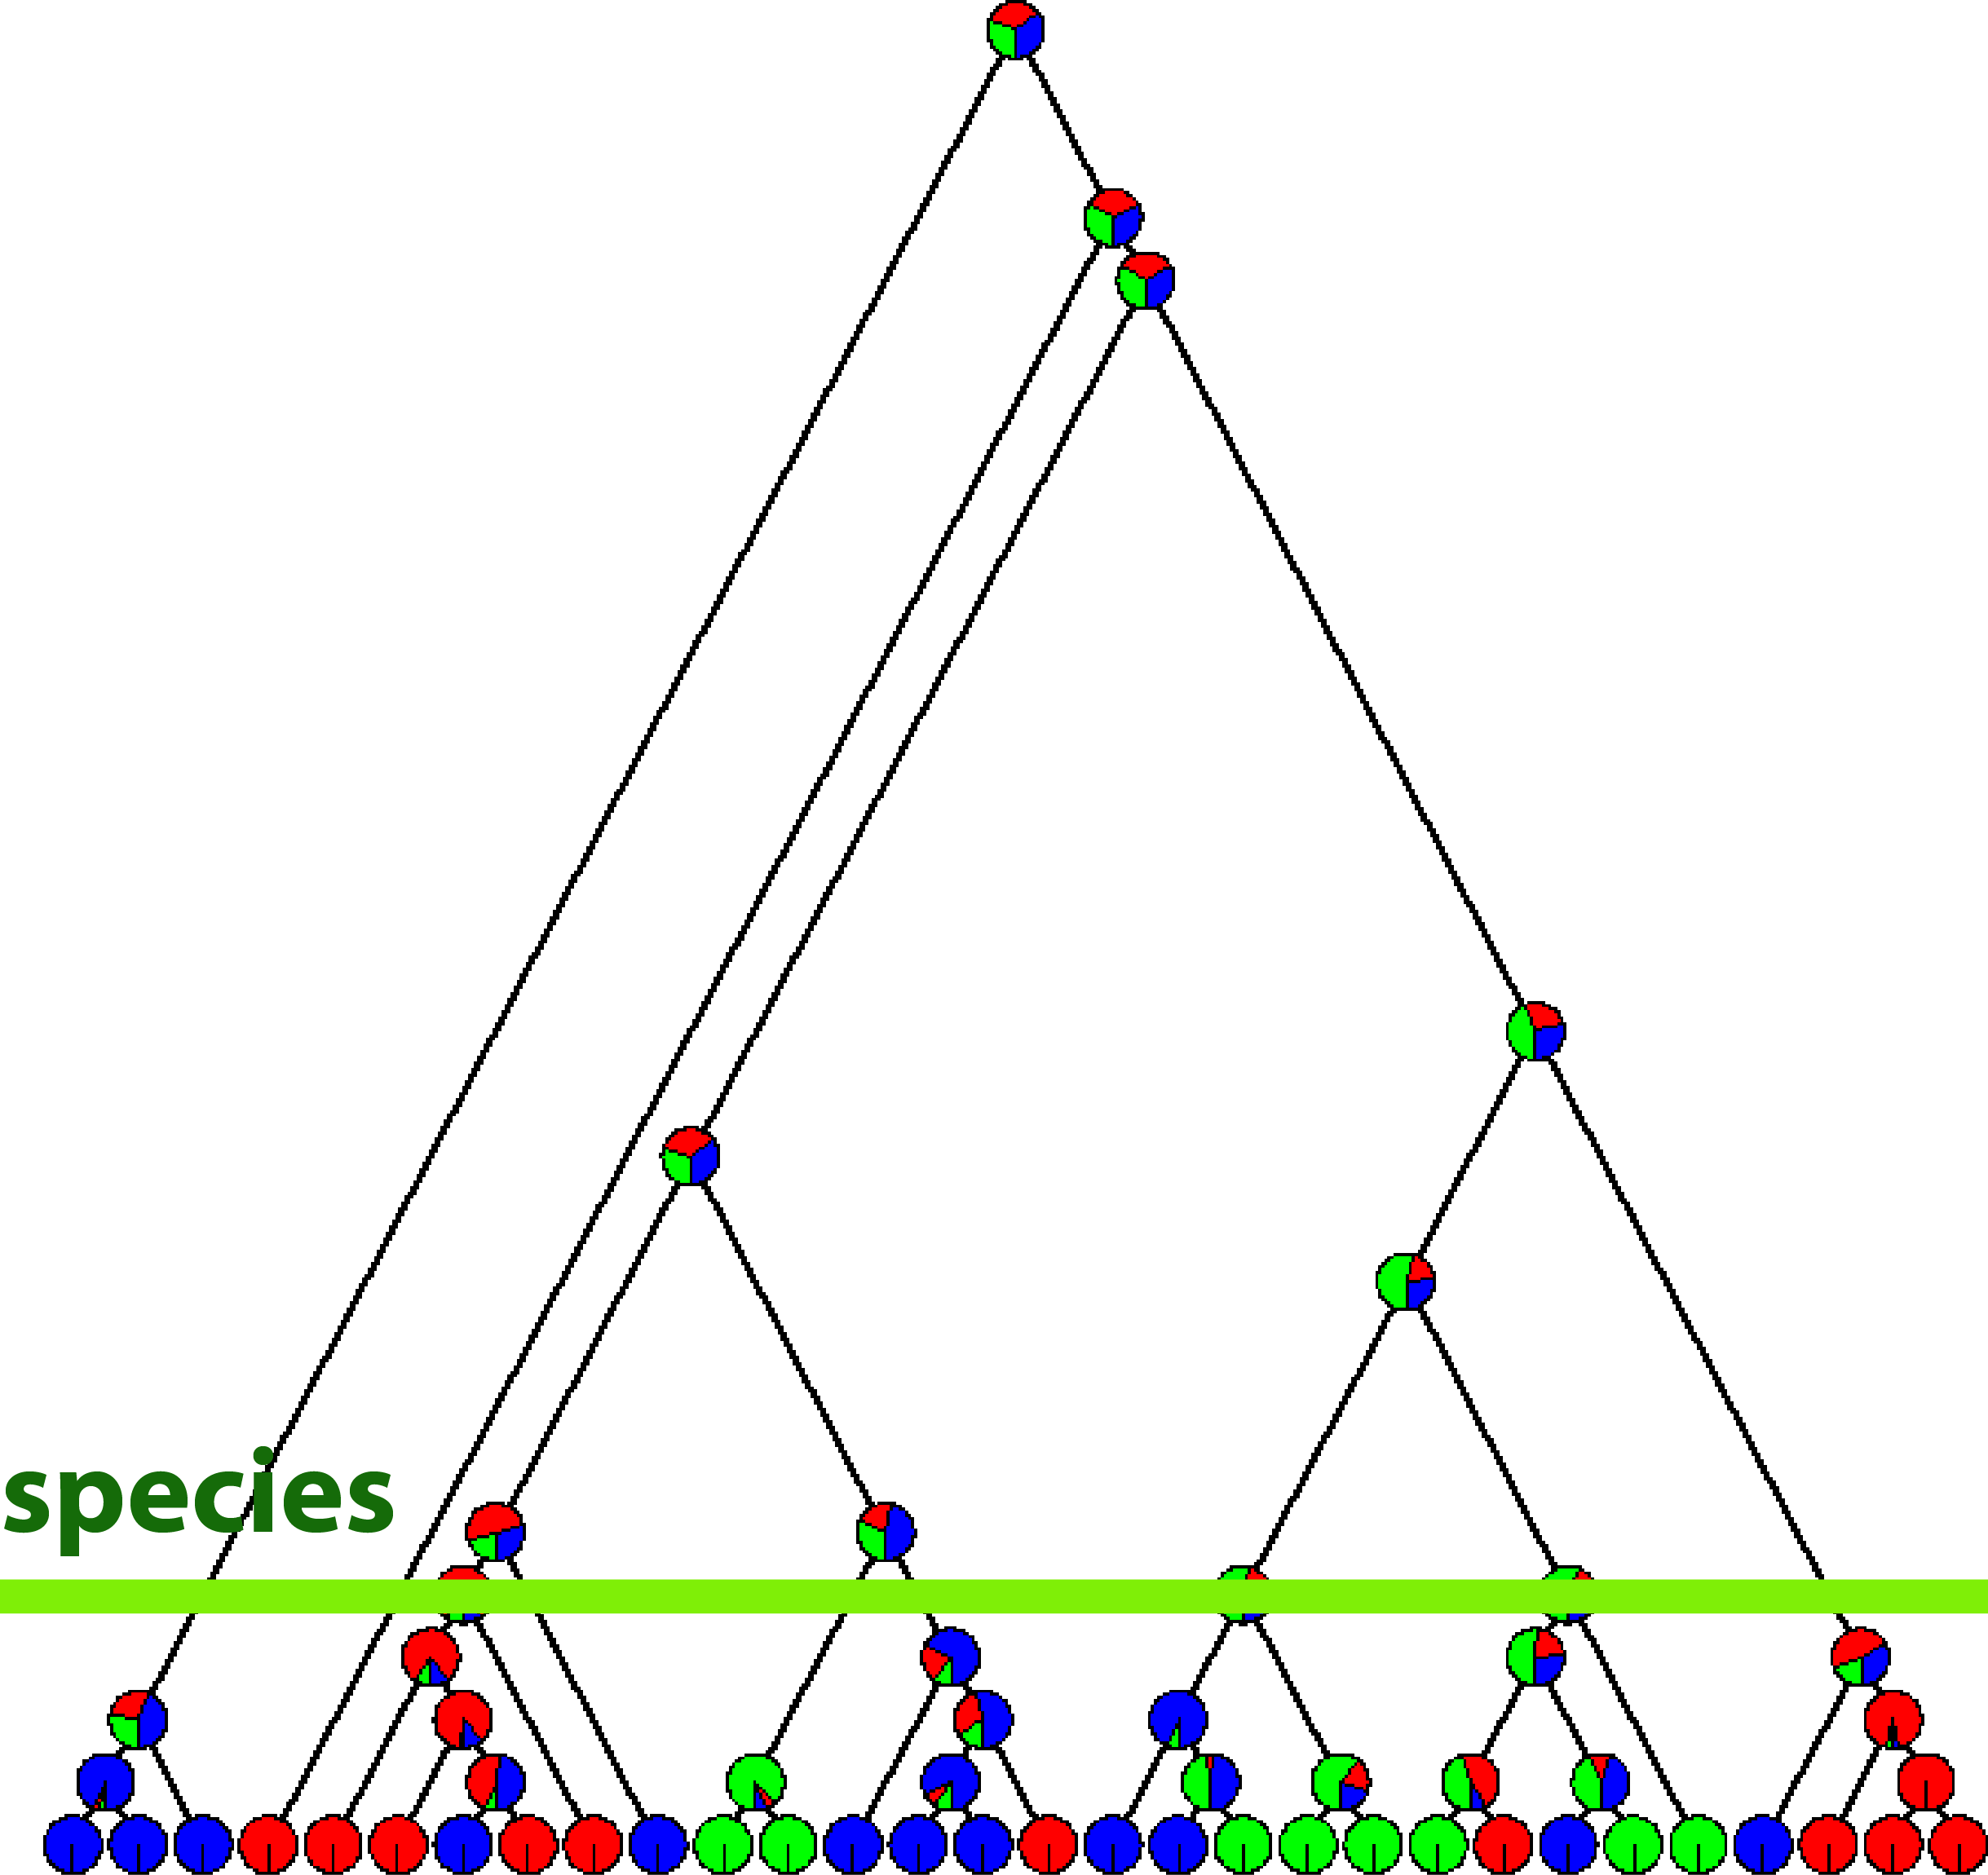
\includegraphics[width=\textwidth]{images/cladogram_species}
    \end{columns}  
\end{frame}

%
\begin{frame}
  \frametitle{Types of comparison}
    \begin{columns}[T] 
      \column{.5\textwidth} 
        \textcolor{RawSienna}{\textbf{Within genera/between species}}
        \begin{itemize}
	  \item what genome features show evidence of selective pressure?
	  \item which species are under selective pressure for which functions?        
        \end{itemize}
      \column{.5\textwidth}
        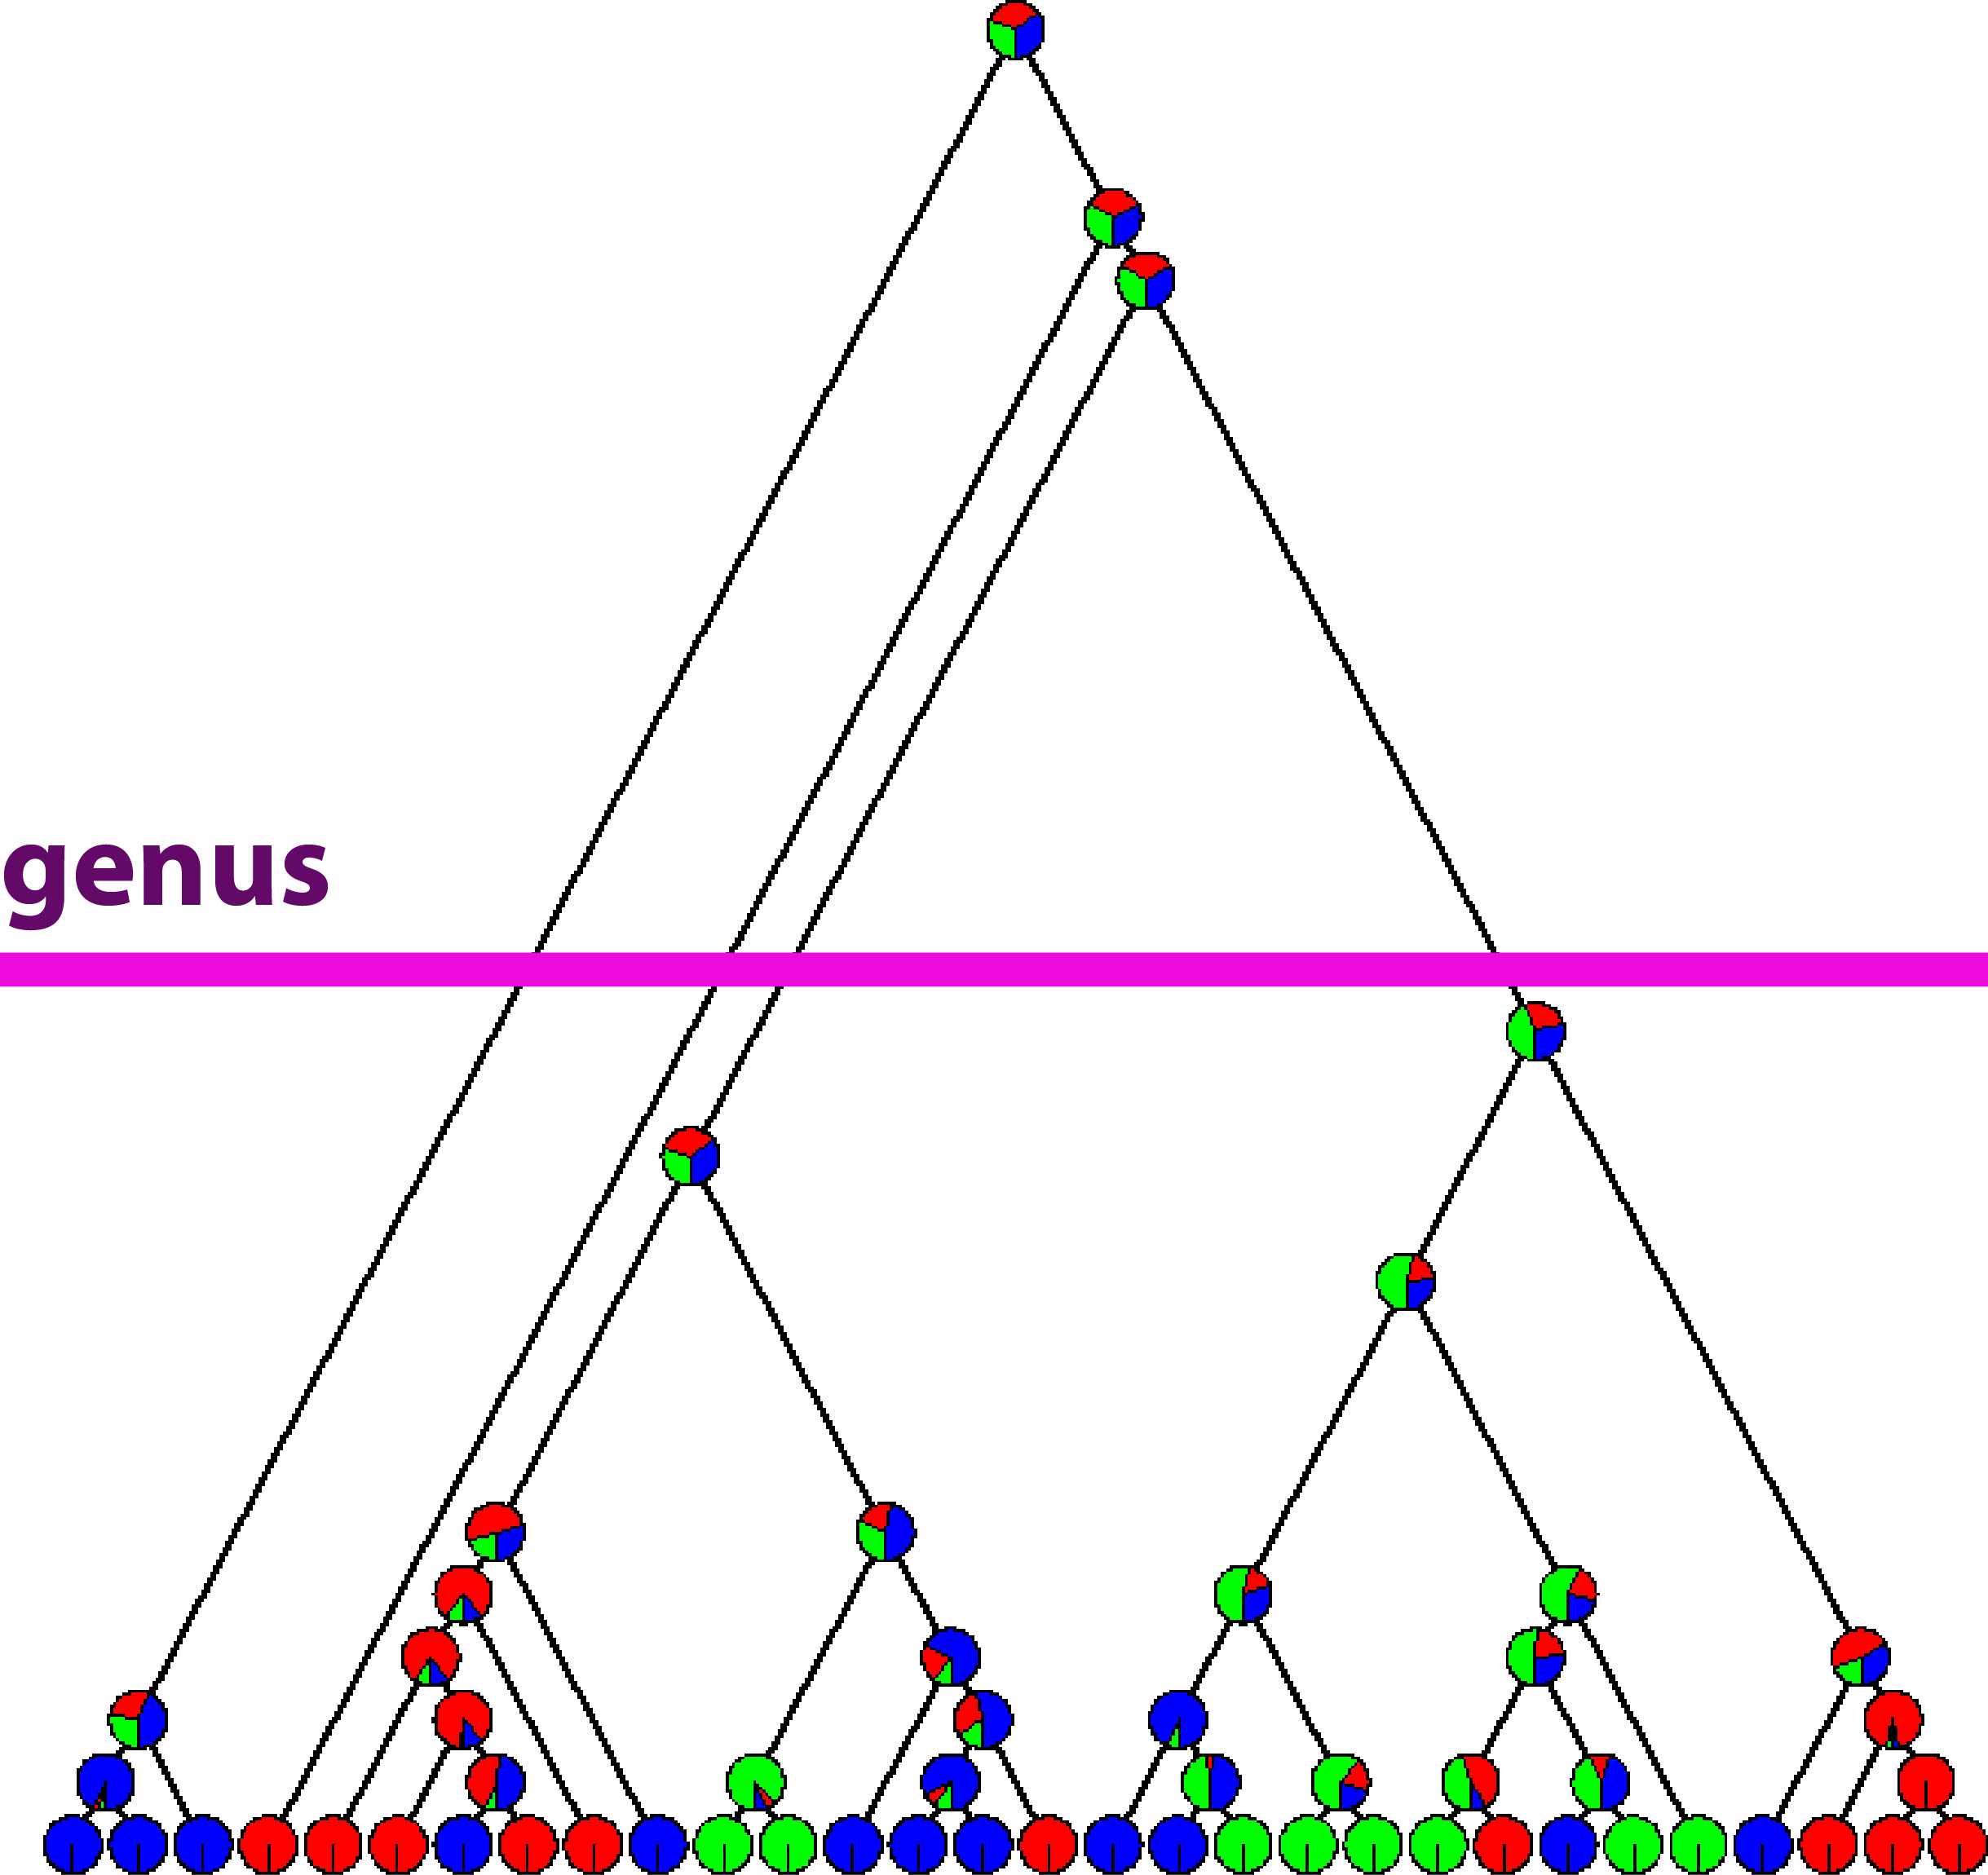
\includegraphics[width=\textwidth]{images/cladogram_genus}
    \end{columns}  
\end{frame}

%
\begin{frame}
  \frametitle{Types of comparison}
    \begin{columns}[T] 
      \column{.5\textwidth} 
        \textcolor{RawSienna}{\textbf{Between subgroups}}
        \begin{itemize}
          \item what are the core set of genome features that define a subgroup or genus?
          \item what functions are present/absent between groups?
        \end{itemize}
      \column{.5\textwidth}
        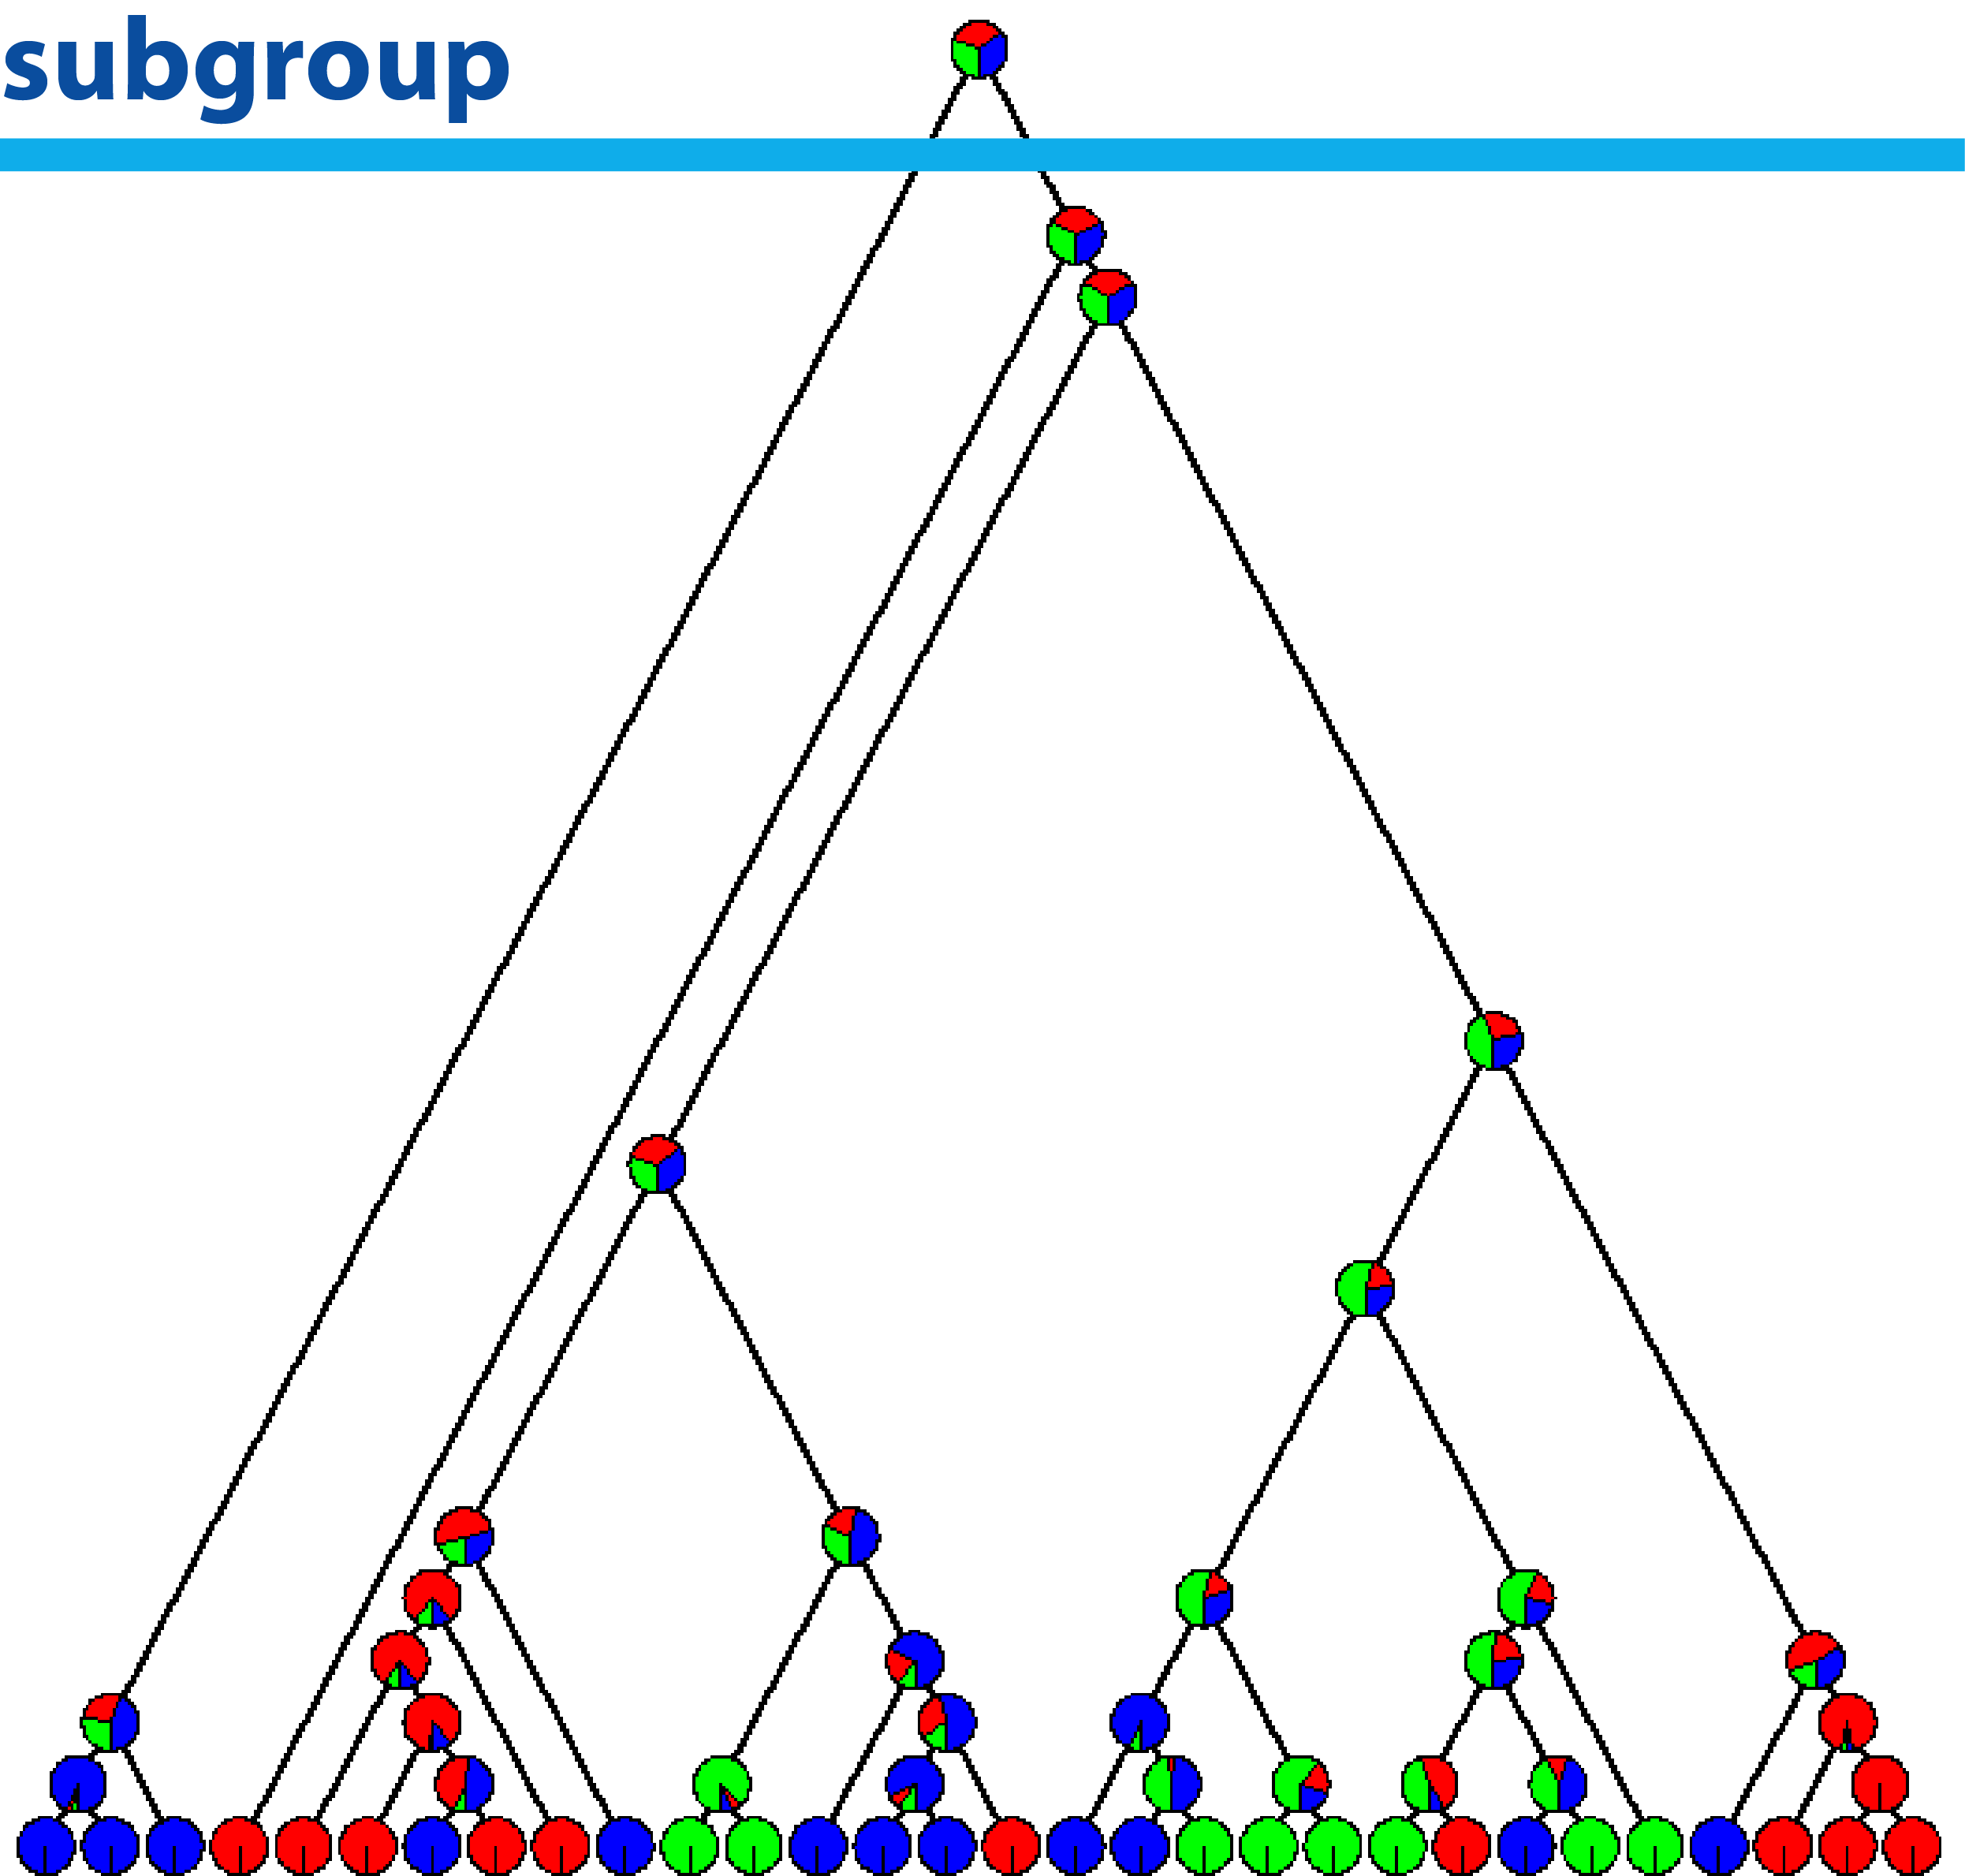
\includegraphics[width=\textwidth]{images/cladogram_subgroup}
    \end{columns}  
\end{frame}